\chapter{Wirtualna rzeczywistość}
\label{chap:pierwszy}



%-------------------------------------------------------
\section{Wprowadzenie}

Interfejs, bo tak nazwana jest płaszczyzna, na której dochodzi do komunikacji między człowiekiem a komputerem, przez wiele lat przechodziła ewolucje – począwszy od wiersza poleceń, poprzez interfejs graficzny, a skończywszy na bezpośredniej komunikacji na poziomie mózg-komputer. Użytkownicy pierwszych interfejsów musieli ówcześnie posiąść wiedzę na temat ich obsługi, gdzie przykładem może być konieczność zaznajomienia się ze składnią tekstową i komendami wykorzystywanymi w danym systemie operacyjnym. Dziś coraz częściej używane są komunikaty przekazane przez człowieka w naturalny i intuicyjny sposób, takie jak gesty wykonywane na ekranach dotykowych smartfonów palcami dłoni, komendy głosowe oraz gesty wykonywane przy pomocy ciała, rozpoznawalne przez kamery i czujniki ruchu  \citep{virtualtech, virtualspeech}.

Za finalny etap ewolucyjny  uważa się całkowitą naturalizację interfejsu – co można częściowo zaobserwować na przykładzie wirtualnej rzeczywistości. Pozwala ona na skrócenie dystansu pomiędzy maszyną a człowiekiem dzięki rozszerzeniu jego zmysłów: słuchu, dotyku i wzroku przy wykorzystaniu technologii informatycznej co pozwala na wykreowanie pewnej wizji rzeczywistości, jednakże w świecie wirtualnym. W ciągu następnych dekad możemy spodziewać się znaczących zmian w naszych działaniach związanych z pracą, rozrywką i komunikacją, a wszystko dzięki rozwojowi wirtualnej rzeczywistości \citep{virtualspeech}.



\section{Definicja, części składowe i systematyzacja wirtualnej rzeczywistości}

Wirtualna rzeczywistość zdefiniowana pod względem funkcjonalności to świat syntetyczny i niestatyczny, czyli taki, który reaguje na dane wejściowe użytkownika - gesty czy polecenia słowne. To z kolei, definiuje kluczową cechę wirtualnej rzeczywistości jaką jest interaktywność w czasie rzeczywistym. Interaktywność oraz siła z jaką VR absorbuje uwagę użytkownika, przyczyniają się do stworzenia uczucia ``zanurzenia'' w tymże świecie, czyli immersji \citep{virtualtech}.

Z powyższego opisu jasno wynika, że rzeczywistość wirtualna jest zarówno interaktywna (ang. interactive) jak i wciągająca (ang. immersive). Istnieje jednak trzecia składowa, bez której VR nie miałoby racji bytu, czyli ludzka wyobraźnia (ang. imagination). Zakres, w jakim aplikacja jest w stanie rozwiązać konkretny problem, czyli stopień, w którym symulacja działa prawidłowo, zależy więc w dużej mierze od ludzkiej wyobraźni. Rzeczywistość wirtualna jest zatem zintegrowanym trio immersji-interakcji-wyobraźni (ang. immersion, interaction, imagination), tak jak to pokazano na rysunku \ref{fig:triangle}, czyli trójkącie trzech ``I'' wirtualnej rzeczywistości \citep{virtualtech}.


\begin{figure}[h]
	\centering
	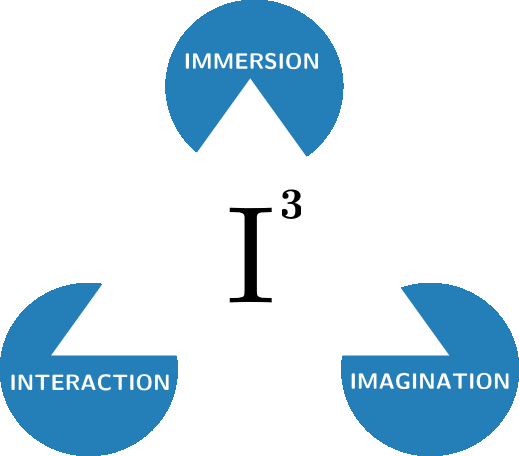
\includegraphics[width=0.6\textwidth]{images/triangle.png}
	\caption{Trzy składowe wirtualnej rzeczywistości.}
	\caption*{Źródło: \citep[s.~5]{virtualtech}.}
	\label{fig:triangle}
\end{figure}

Składowa jaką jest wyobraźnia, odnosi się do zdolności umysłu do postrzegania zasugerowanych, lecz nieistniejących rzeczy. Stąd trójkąt na rysunku 1 jest widoczny dla czytelnika, ale istnieje tylko w jego wyobraźni \citep{virtualtech}.

W celu ujednolicenia, każde kolejne odniesienie do wirtualnej rzeczywistości będzie bazowało na następującej definicji. Rzeczywistość wirtualna to immersyjna, interaktywna rzeczywistość symulowana komputerowo, która dzięki zaawansowanym urządzeniom wejścia i wyjścia tworzy złudzenie fizycznego środowiska, nie istniejącego w prawdziwym świecie fizycznym. Środowiska VR są zazwyczaj odcięte od tego świata w tym sensie, że cyfrowe środowiska, które powstają są całkowicie nowe - chociaż mogą być oparte na prawdziwych miejscach (takich jak szczyt Mount Everest) lub wymyślonych (takich jak podwodne miasto Atlantyda). Osoba korzystająca z wirtualnej rzeczywistości może rozglądać się po sztucznym świecie, poruszać się po nim, a także wchodzić w interakcję z wirtualnymi funkcjami i przedmiotami \citep{virtualfor}.

Rzeczywistość wirtualna jest często używana jako pojęcie ogólne dla wszelkiego rodzaju doświadczeń mocno absorbujących uwagę użytkownika, w tym wielu powiązanych terminów, takich jak rzeczywistość rozszerzona (ang. augumented reality, AR), rzeczywistość mieszana (ang. mixed reality, MR)  i rzeczywistość rozszerzona (ang. extended reality, XR) \citep{virtualfor}. W celu wyjaśnienia, czym dokładnie jest wirtualna rzeczywistość i czym różni się od pochodnych jej technologii, zostaną one umieszczone na skali Paula Miligrama, nazwanej kontinuum wirtualności, którą przedstawia rysunek \ref{fig:continuum}.

\begin{figure}[h]
	\centering
	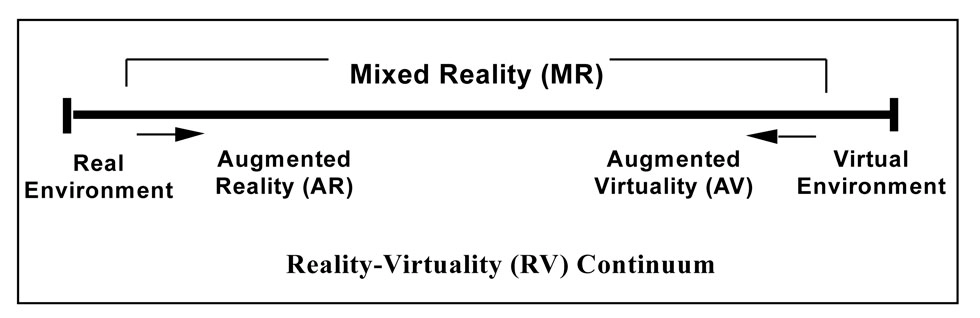
\includegraphics[width=1\textwidth]{images/2.spektrum.png}
	\caption{Kontinuum wirtualności.}
	\caption*{Źródło: \citep[s.~14]{virtualfor}.}
	\label{fig:continuum}
\end{figure}

Kontinuum wirtualności to skala używana do pomiaru poziomu rzeczywistości lub wirtualności konkretnych technologii. Na jednym końcu skali poziom jest w pełni realny, a na drugim całkowicie wirtualny. XR obejmuje pełne spektrum tej skali. Warto dodać, że MR oraz AR zostały rozdzielone, pomimo tego, że często określeń tych używa się synonimicznie. Niniejszy rozdział skupiać się będzie natomiast na głównych dwóch obszarach: VR i AR, które pokrywają większość scenariuszy związanych z rozszerzoną rzeczywistością.  Wirtualna rzeczywistość będzie używana w stosunku do kombinacji sprzętu i oprogramowania, które tworzy całkowicie nowe, cyfrowe symulacje. Natomiast rzeczywistość rozszerzona odnosić się będzie do dowolnego, istniejącego środowiska fizycznego jakie zostało wzbogacono o elementy cyfrowe, które z kolei nie muszą z nim bezpośrednio oddziaływać ani być interaktywne \citep{virtualfor}.

Rzeczywistość rozszerzona AR to jeden ze sposobów oglądania prawdziwego świata w sposób bezpośredni lub za pomocą urządzeń elektronicznych, takich jak kamera, która tworzy wizualizację świata fizycznego i ``rozszerza'' go za pomocą generowanych komputerowo danych graficznych, dźwiękowych i filmowych. AR różni się od VR tym, że AR powiększa istniejącą już fizycznie scenę o dodatkowe elementy, zamiast tworzyć całkowicie nową od podstaw. Pierwotnie uważano, że w AR dwa środowiska: fizyczne i syntetyczne nie mogą się ze sobą komunikować. W ostatnich latach definicja AR przybrała jednak inną formę i jest utożsamiana z rzeczywistością mieszaną, czyli taką, w której może zachodzić interakcja między światem rzeczywistym a cyfrowo rozszerzonym \citep{virtualfor}.

Porównanie zasady działania różnych typów rozszerzonej rzeczywistości przedstawia rysunek \ref{fig:vr-ar-mr}. Kolor zielony odwzorowuje obraz wirtualny, natomiast odcienie szarości przedstawiają świat fizyczny.


\begin{figure}[ht]
	\centering
	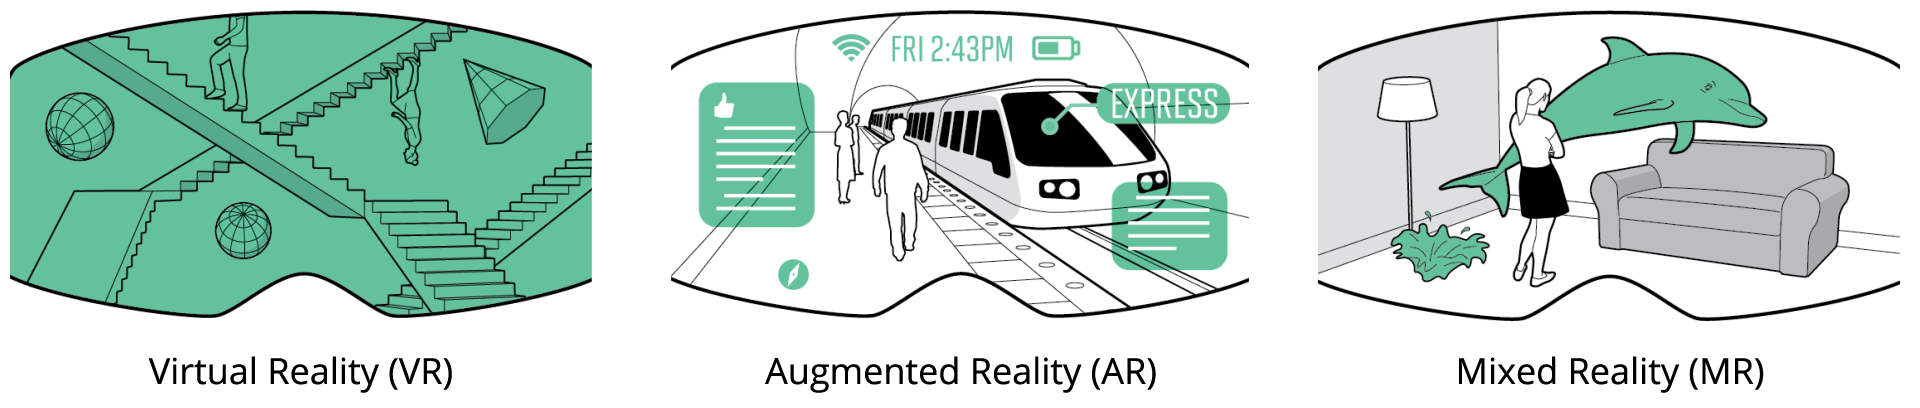
\includegraphics[width=1\textwidth]{images/1.xr-comparision.png}
	\caption{Porównanie VR, AR oraz MR.}
	\caption*{Źródło: https://www.cadcompany.nl/blog/vr-ar-en-mr-verschillen/}
	\caption*{Data dostępu: 15.02.2020.}
	\label{fig:vr-ar-mr}
\end{figure}

Rzeczywistość mieszana MR może przybrać różne formy i skłaniać się bardziej w stronę AR lub VR. Rzeczywistość mieszana, której podstawą jest AR, nie jest pasywnie nakładana na świat rzeczywisty, lecz zachowuje się jakby była częścią tego świata i wchodzi z nim w interakcje. Obiekty cyfrowe wyglądają tak, jakby istniały w prawdziwej przestrzeni. Przykładem może być umieszczona na stoliku do kawy cyfrowa rakieta, która rozpoczyna swoją misję kosmiczną lub cyfrowa piłka, która odbija się od ścian świata rzeczywistego. W innej wersji natomiast ukazuje się całkowicie cyfrowe środowisko lecz powiązane z otaczającymi użytkownika obiektami świata rzeczywistego, tak więc na przykład fizyczne, drewniane krzesła mogą mieć swoje odwzorowanie jako drzewa w cyfrowym świecie – jest to MR oparty na VR \citep{virtualfor}.

Rozszerzona wirtualność AV (z ang. Augumented virtuality), nazywana także połączoną rzeczywistością jest zasadniczo odwrotnością AR. Rozszerzona wirtualność dotyczy środowiska cyfrowego, w którym istnieje pewna integracja obiektów rzeczywistych poprzez strumieniowe przesyłanie video do środowiska wirtualnego lub tworzenia cyfrowej reprezentacji 3D istniejącego obiektu fizycznego \citep{virtualfor}.



%-------------------------------------------------------
\section{Ewolucja wirtualnej rzeczywistości}


%-------------------------------------------------------
\subsection{Narodziny}

Biorąc pod uwagę VR jako narzędzie do tworzenia iluzji – przeniesienia użytkownika w miejsce, w którym nie jest fizycznie to jako tego najwcześniejszą próbę możemy traktować 360 stopniowe malowidła ścienne lub panoramiczne obrazy z XIX wieku. Ich celem było wypełnienie całego pola widzenia obserwatora, sprawiając przy tym, że czuł się on ``zanurzony'' w wydarzeniu lub scenie oddanej na malowidle \citep{interactivemedia}.

Badania opublikowane w 1838 roku przez Charlesa Wheatstone’a wykazały, że ludzki mózg przetwarza dwa dwuwymiarowe obrazy z każdego oka w jeden, pojedynczy obiekt o trzech wymiarach. Stąd oglądanie dwóch zdjęć (jedno widoczne dla jednego oka, a drugie – podobne lecz nieidentyczne dla drugiego) za pomocą stereoskopu zapewniało użytkownikowi poczucie głębi i zanurzenia. Późniejszy rozwój popularnego stereoskopu View-Master opatentowanego w 1939 roku, dało początek dzisiejszym goglom VR \citep{interactivemedia}.

Wirtualna rzeczywistość choć dopiero teraz zyskuje na popularności, nie jest wynalazkiem XXI wieku, a jej historia sięga lat 50 ubiegłego stulecia. Za ojca VR uważany jest operator filmowy Morton Heiling, który to w 1962 roku zaprezentował maszynę o nazwie ``Sensorama'', którego schemat widnieje na rysunku \ref{fig:sensorama1}, a zdjęcie zostało przedstawione na rysunku \ref{fig:sensorama2}.  Było to urządzenie mechaniczne, którego zadaniem było symulowanie jazdy motocyklem przez Nowy Jork \citep{determinants}. Doświadczenie to polegało na jeździe wyimaginowanym motorem podczas oglądania krótkich ujęć filmów z ulic Nowego Jorku. W celu zwiększenia realności całego doświadczenia, symulowano podmuchy wiatru, zmiany kierunku jazdy, hałas oraz zapachy spotykane w mieście – od spalin po nowojorską pizzę, w zależności od miejsca, w jakim aktualnie znajdował się użytkownik. W systemie Sensorama brakowało jednak głównego elementu nowoczesnego systemu rzeczywistości wirtualnej: reakcji opartej na działaniach użytkownika \citep{virtualdev}.


\begin{figure}[ht]
    \centering
    \begin{minipage}{0.45\textwidth}
        \centering
        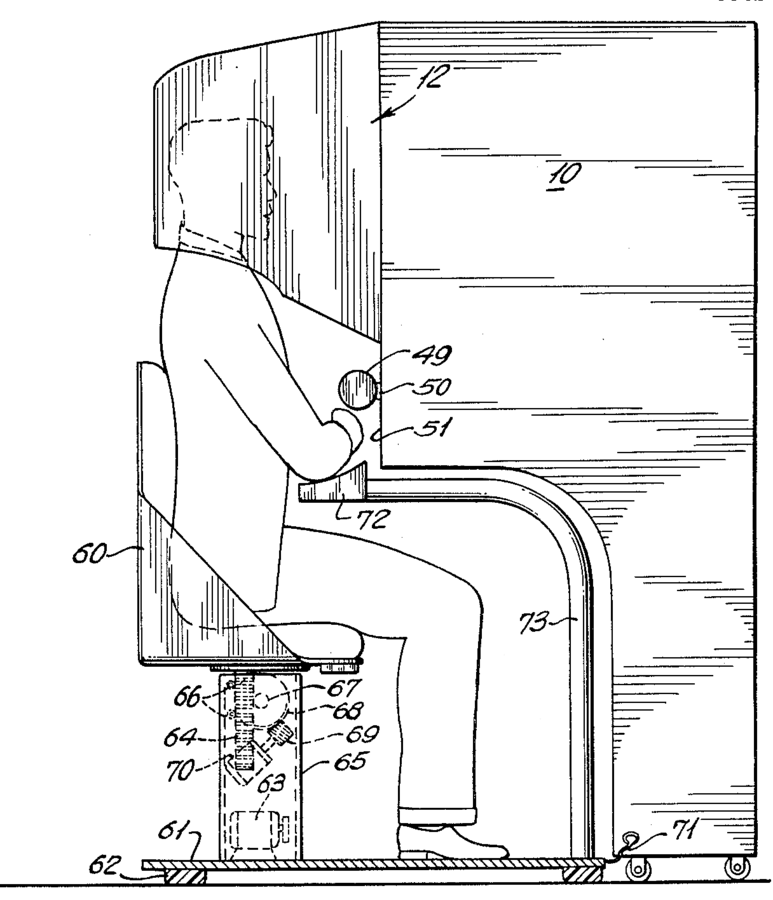
\includegraphics[width=0.9\textwidth]{images/sensorama1.png} % first figure itself
        \caption{Schemat Sensoramy w przekroju bocznym (zdjęcie z patentu USA nr #3050870).}
        \caption*{Źródło: https://smattes.com/article
        /47/sensorama}
        \caption*{Data dostępu: 15.02.2020.}
        \label{fig:sensorama1}
    \end{minipage}\hfill
    \begin{minipage}{0.45\textwidth}
        \centering
        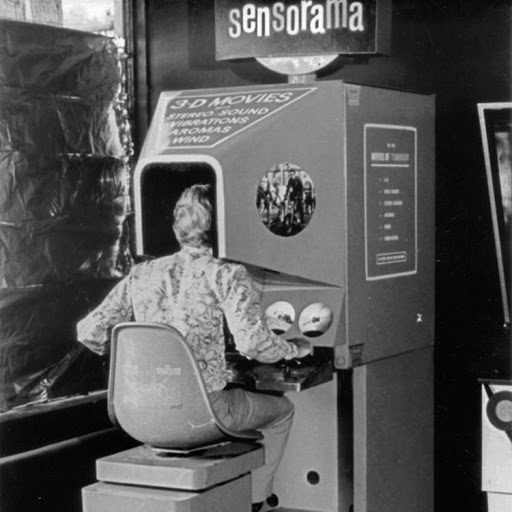
\includegraphics[width=0.9\textwidth]{images/sensorama2.jpg} % second figure itself
        \caption{Sensorama - pierwsze urządzenie wykorzystujące VR.}
        \caption*{Źródło: https://www.researchgate.net
        /figure/Sensorama-From-web-page-
        InventorVR-retrieved-in-March-2014-from\_fig1\_263388241}
        \caption*{Data dostępu: 15.02.2020.}
        \label{fig:sensorama2}
    \end{minipage}
\end{figure}


%-------------------------------------------------------
\subsection{Rozwój}

Krótko po wynalezieniu Sensoramy, Heilig opatentował również maskę Telesphere, pierwszy w historii wyświetlacz montowany na głowie HMD (ang. head-mounted display), czyli tak zwany hełm wideo, który zapewniał stereoskopowy obraz 3D i dźwięk stereo. Zestaw ten był nadal nieinteraktywny, choć zewnętrznie przypominał dzisiejsze okulary VR \citep{website:virtualspeech}.

W roku 1968 Ivan Sutherland, profesor Harvardu w dziedzinie informatyki, wynalazł pierwszy interaktywny hełm wideo, który był podłączony do komputera. System Sutherlanda to duży sprzęt, podwieszany przy suficie, który nosił nazwę ``Miecz Damoklesa''. Obejmował on hełm wideo oraz elementy, które mechanicznie śledziły głowę za pomocą szpulowych zwijanych kabli oraz program komputerowy, który w prosty sposób w formie trójwymiarowej generował prymitywne pokoje lub obiekty szkieletowe jak na przykład cząsteczka wody.  Sutherland w późniejszym czasie opracował zaawansowany sprzęt do renderowania grafiki w czasie rzeczywistym dla społeczności pilotów korzystających z symulatorów lotów, już jako  współzałożyciel Evans i Sutherland Computer Corporation (E&S) \citep{virtualdev}.


Po demonstracji Sutherlanda w laboratoriach uniwersyteckich, instytucjach rządowych i wojskowych, a później w sektorze komercyjnym, podjęto szereg prac badawczo-rozwojowych. W społeczności akademickiej badacz z University of Wisconsin, Myron Krueger eksperymentował z rozszerzoną rzeczywistością, czego wynikiem było powstanie systemu nazwanego ``Videoplace''. Systemy Kruegera również różniły się od pracy Sutherlanda tym, że wykorzystywał sygnały wejściowe z kamery wideo do śledzenia ruchów użytkownika. Videoplace było miejscem, w skład którego wchodziły zaciemnione pomieszczenia z zainstalowanymi na ścianach ekranami wideo, które otaczały użytkownika. Odbiorcy mogli zobaczyć wygenerowane przez komputer sylwetki naśladujące ich ruchy i działania - ruchy użytkowników były rejestrowane w kamerze i przenoszone na wirtualną postać. Ponadto użytkownicy różnych pokoi mogli wchodzić w interakcje z innymi użytkownikami w wirtualnym świecie, co powoli prowadziło do wniosków, że komunikacja w wirtualnym świecie jest możliwa, nawet jeśli dwie osoby nie są fizycznie blisko \citep{website:virtualspeech}.


W czasie, gdy Ivan Sutherland pracował nad projektem „Miecz Damoklesa”, inżynier wojskowy Thomas Furness opracowywał swój prywatny projekt - ``Super Kokpit''. Furness kontynuował prace nad projektem do lat osiemdziesiątych, w wyniku czego kokpit szkoleniowy był w stanie wyświetlać wygenerowane komputerowo mapy 3D, zdjęcia w podczerwieni i obrazy radarowe, a także dane samolotu w przestrzeni 3D w czasie rzeczywistym \citep{website:digitaltrends}.

W roku 1978 Massachusetts Institute of Technology (MIT) opracowało Aspen Movie Map, która znacząco przypominała dzisiejszą funkcję ``street view'' oferowaną przez Google Maps. Program ten pozwolił użytkownikowi na wirtualny spacer przez miasto Aspen (Kolorado) w trzech trybach: letnim, zimowym i wyświetlającym wielokąty. Doświadczenie to zostało stworzone na podstawie zdjęć z samochodu jadącego przez miasto. Chociaż projekt ten nie wykorzystywał komponentu hełmu wirtualnego,  w sposób innowacyjny wykorzystano interaktywność z perspektywy pierwszej osoby i ukazano w jak prosty sposób VR można wykorzystać do ``wirtualnego przeniesienia'' ludzi w inne miejsce na Ziemi \citep{website:digitaltrends}.

Rękawice do śledzenia palców dla VR, zwane rękawiczkami ``Sayre'' zostały wynalezione przez Daniela Sandina i Thomasa DeFanti. Rękawice były podłączone do systemu komputerowego i monitorowały ruchy dłoni za pomocą emiterów światła i fotokomórek w palcach rękawic. Kiedy użytkownik poruszał palcami, ilość światła padającego na fotokomórkę zmieniała się, co następnie przekształcało ruchy palców w sygnały elektryczne. Był to prekursor ``rękawic danych'', które stały się w późniejszym czasie ważną częścią wczesnej rzeczywistości wirtualnej \citep{website:virtualspeech}.

Pomimo prężnego rozwoju VR wciąż nie było terminu opisującego tę dziedzinę. Wszystko zmieniło się w 1987 roku, gdy Jaron Lanier, założyciel laboratorium programowania wizualnego (VPL), wymyślił termin ``rzeczywistość wirtualna''. W późniejszym czasie, dzięki swojej firmie VPL Research Jaron opracował gamę sprzętu do rzeczywistości wirtualnej, w tym Dataglove (wraz z Tomem Zimmermanem) i montowany na głowie wyświetlacz  EyePhone. Była to pierwsza firma, która sprzedawała gogle oraz rękawice do obsługi wirtualnej rzeczywistości. Miało to znaczący wpływ na rozwój w dziedzinie dotykowej rzeczywistości \citep{website:learng2, interactivemedia}. Rysunek \ref{fig:eyephone} przedstawia rękawice Dataglove oraz headset Eyephone podczas użytkowania.

\begin{figure}[ht]
	\centering
	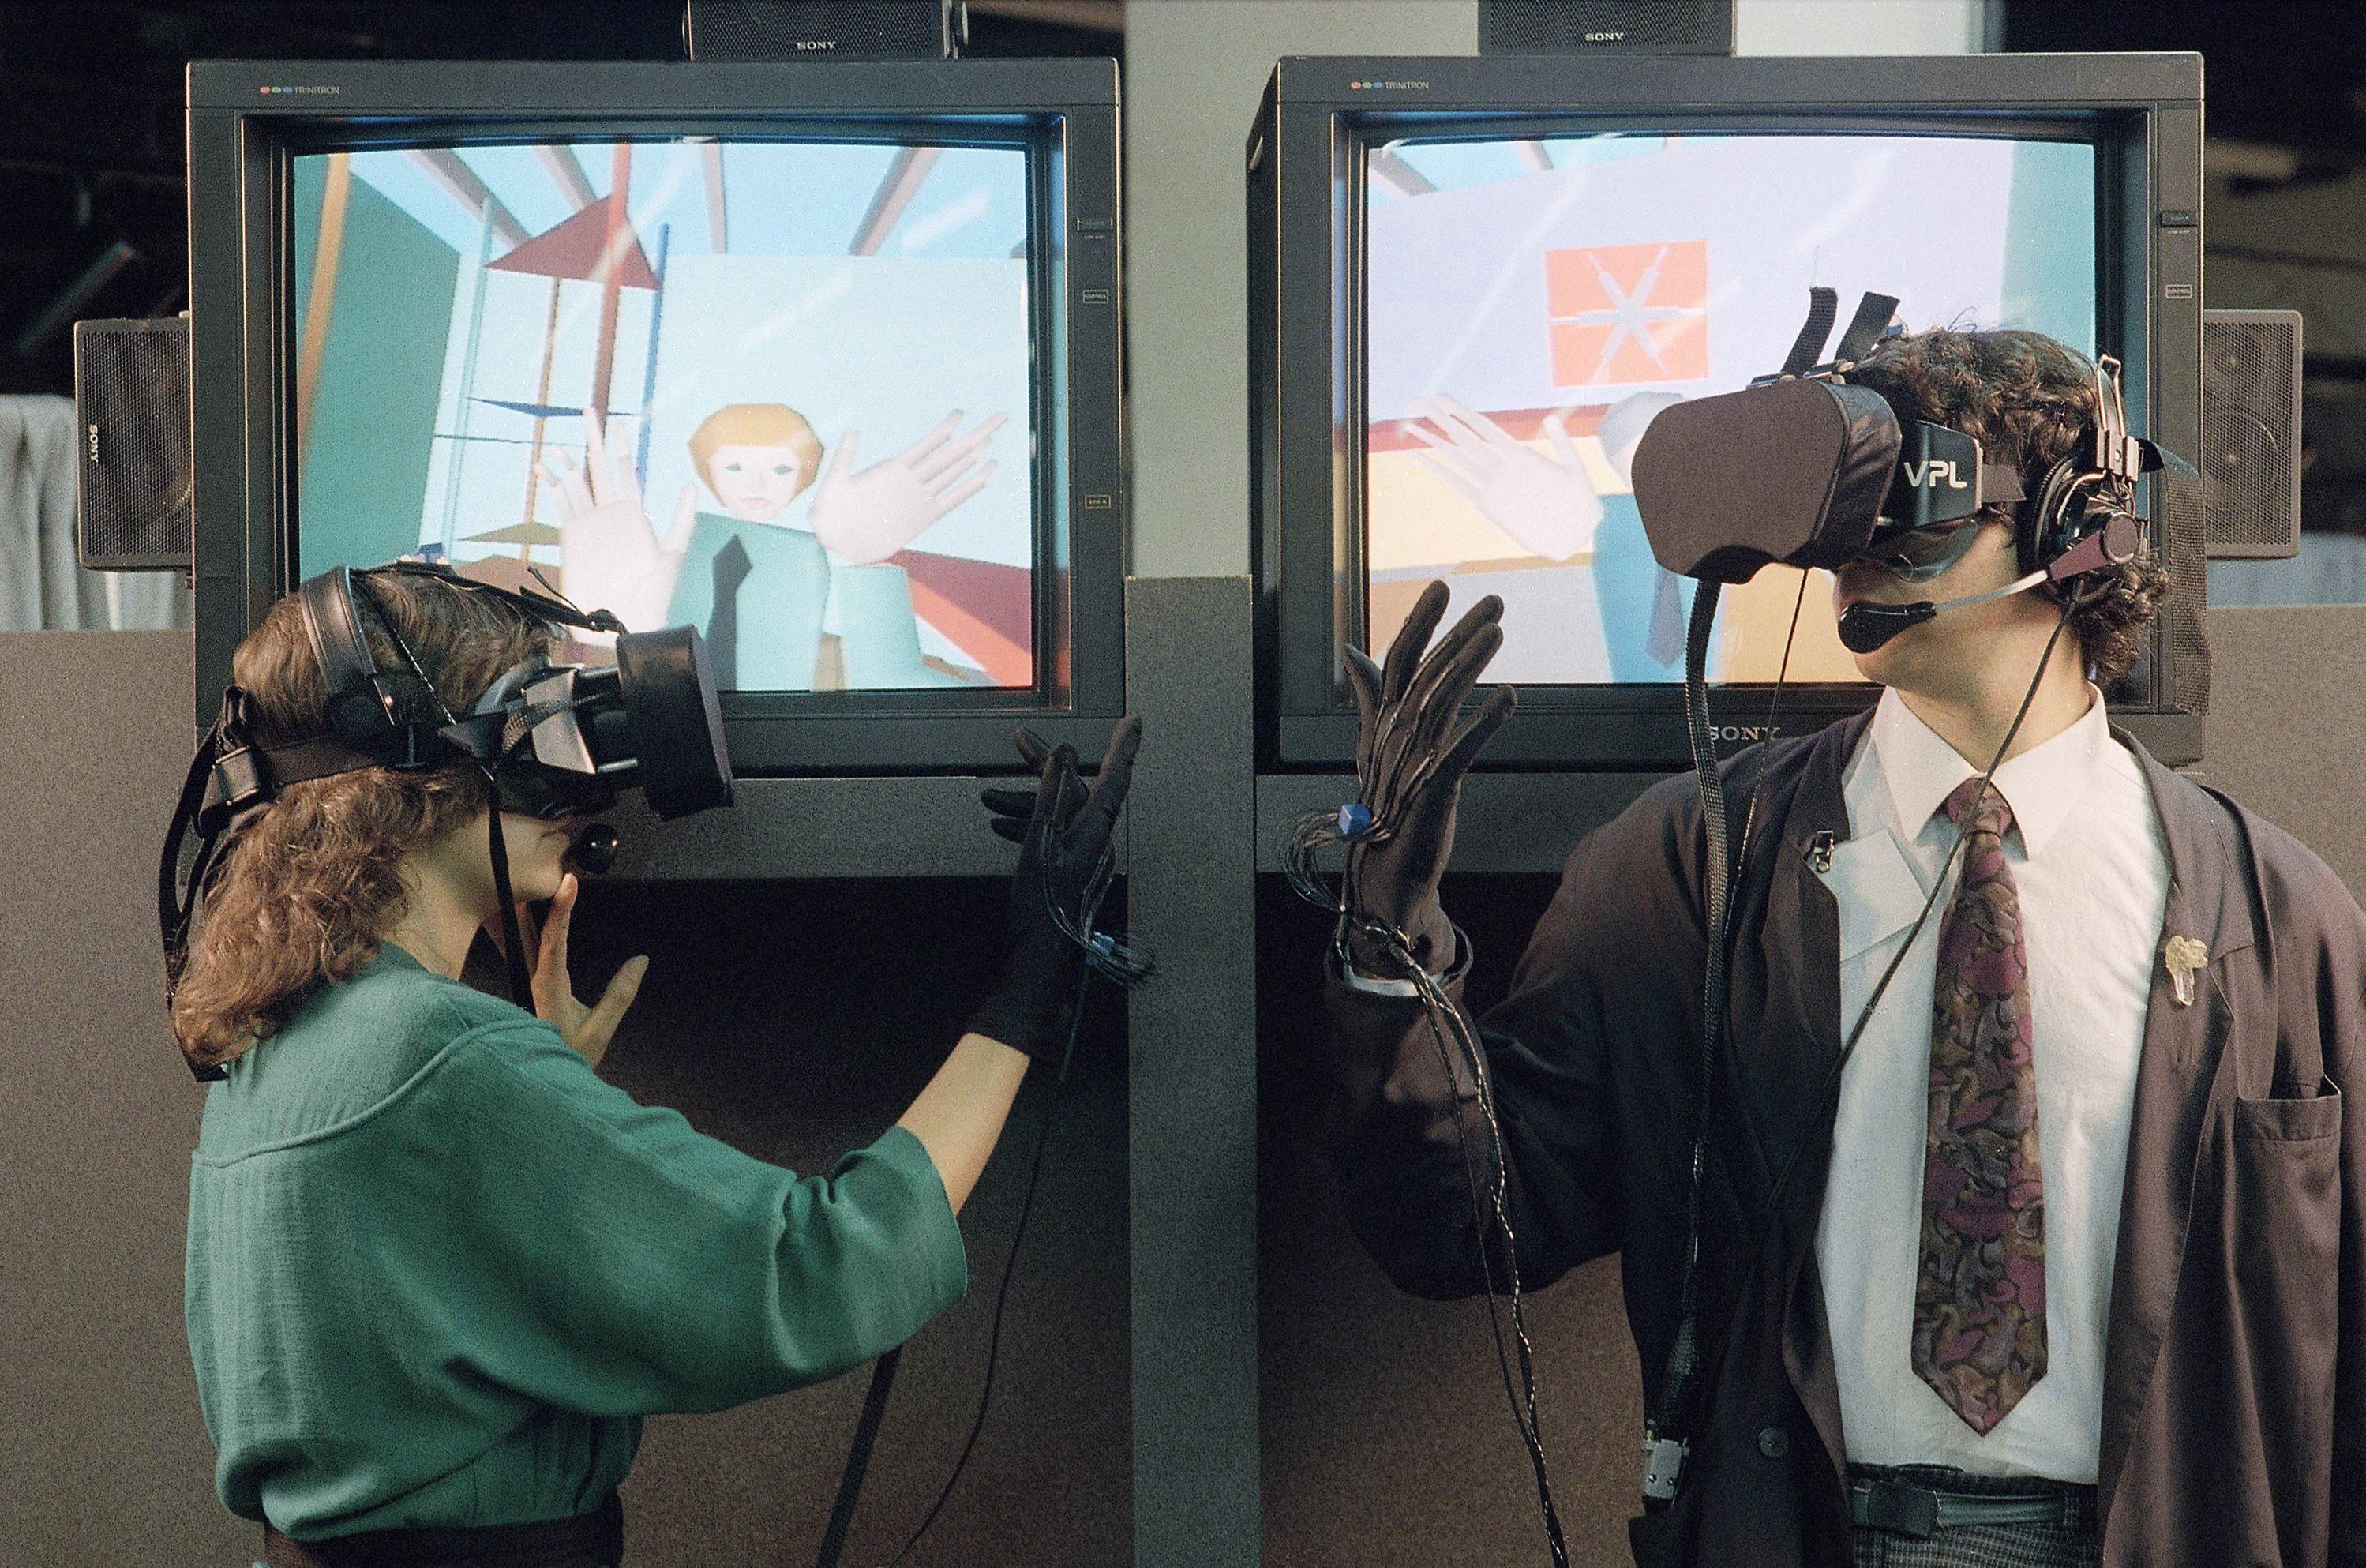
\includegraphics[width=0.7\textwidth]{images/jaron.jpg}
	\caption{Rękawice Dataglove oraz headset Eyephone w trakcie użycia.}
	\caption*{Źródło: https://flashbak.com/jaron-laniers-eyephone-head
	-and-glove-virtual-reality-in-the-1980s-26180/}
	\caption*{Data dostępu: 20.02.2020.}
	\label{fig:eyephone}
\end{figure}

Rok 1991 był przełomowy dla systemów VR dostarczających rozrywkę. Grupa Virtuality zaczęła dystrybuować automaty do gier VR o nazwie ``Virtuality'', w których gracze mogli grać w świecie gier 3D. Był to pierwszy masowo produkowany system rozrywki VR. Virtuality zawierała stereoskopowe okulary VR, które generowały obrazy 3D w czasie rzeczywistym. Niektóre z maszyn mogły być podłączone wspólnie, pozwalając przy tym na grę w trybie wieloosobowym \citep{website:virtualspeech}.

W 1993 SEGA ogłosiła, że pracuje nad zestawem słuchawkowym SEGA VR, który będzie dostępny dla ogółu społeczeństwa. Ten zestaw słuchawkowy miał być przeznaczony do gier zręcznościowych i konsoli Mega Drive. Wyglądał jak przyłbica dzięki wpływom popularnych wtedy filmów, takich jak RoboCop. W wizjerze umieszczono wyświetlacze LCD, a także słuchawki stereo i czujniki do śledzenia ruchu głowy. Jednak projekt ten nigdy nie został wydany, choć stworzono dla niego cztery gry. Jednym z wyjaśnień jakie ogłosiła firma SEGA, była ich obawa przed utratą zdrowia użytkowników, ponieważ efekt VR był zbyt realistyczny. Wydaje się to jednak mało prawdopodobne ze względu na ograniczoną moc obliczeniową w tamtych latach \citep{website:virtualspeech}.

W roku 1997 rozpoczęto terapie w leczeniu zespołu stresu pourazowego (ang. Posttraumatic Stress Disorder, PTSD) u weteranów wojennych. Do dnia dzisiejszego jest to nadal jeden z kluczowych obszarów leczenia i badań PTSD. Technologia VR dała terapeutom niezrównaną kontrolę nad tym, co pacjenci widzą i czego doświadczają \citep{interactivemedia}.


%-------------------------------------------------------
\subsection{Lata współczesne i prognozy na przyszłość}

Prawdziwy przełom nastąpił w roku 2010. Przedsiębiorca Palem Luckey był zawiedziony zestawami VR dostępnymi na rynku. Według jego opinii były zbyt drogie, ciężkie oraz miały małe pole widzenia, a opóźnienia miedzy interakcją użytkownika a odpowiedzią komputera były zbyt długie. Luckey zbudował serie prototypów zestawów VR, koncentrując się przy tym na stworzeniu taniego zestawu o niskim opóźnieniu, ale z dużym polem widzenia oraz wygodnym w użytku. Jego jednostka szóstej generacji została nazwana Oculus Rift Development Kit 1 i zaoferował ją na platformie Kickstarter, pozwalającej na finansowanie przez użytkowników projektów z różnych dziedzin życia. Zbiórka pieniędzy na rzecz projektu odniosła ogromny sukces, przynosząc 2,4 miliona dolarów, prawie 980 procent pierwotnego celu. Co ważniejsze, kampania Kickstarter przyczyniła się do wzrostu zainteresowania VR na rynku konsumenckim do rekordowego poziomu \citep{virtualfor}. Porównanie pierwszej i najnowszej wersji zestawu Oculus przedstawiono na rysunku \ref{fig:rift} i rysunku \ref{fig:quest}.

\begin{figure}[ht]
    \centering
    \begin{minipage}{0.45\textwidth}
        \centering
        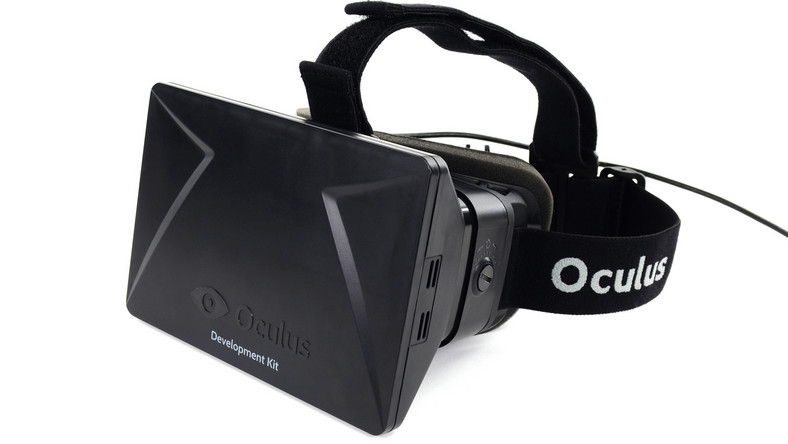
\includegraphics[width=0.9\textwidth]{images/oculusold.jpg} % first figure itself
        \caption{Zestaw Oculus Rift Development Kit 1 z roku 2010.}
        \caption*{Źródło: https://www.ifixit.com/Device
        /Oculus\_Rift\_DK1}
        \caption*{Data dostępu: 25.02.2020.}
        \label{fig:rift}
    \end{minipage}\hfill
    \begin{minipage}{0.45\textwidth}
        \centering
        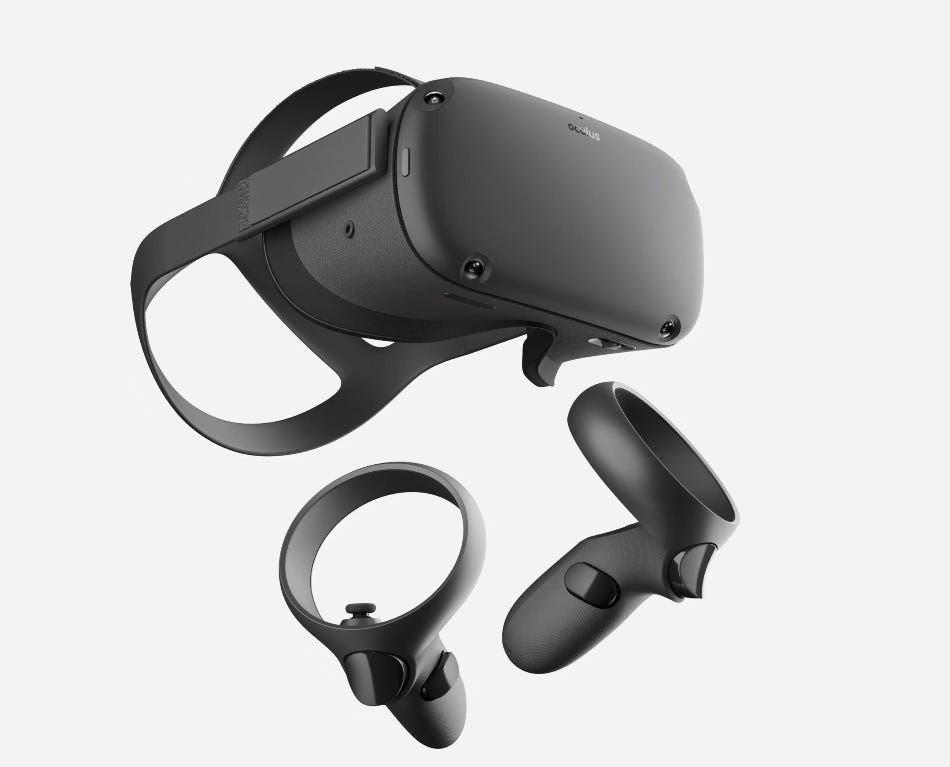
\includegraphics[width=0.9\textwidth]{images/oculusquest.jpg} % second figure itself
        \caption{Zestaw Oculus Quest z roku 2019.}
        \caption*{Źródło: https://i.insider.com/
        5df1222cfd9db23851669bd2?width=1100&
        format=jpeg&auto=webp}
        \caption*{Data dostępu: 25.02.2020.}
        \label{fig:quest}
    \end{minipage}
\end{figure}

Firma została zakupiona przez Facebook za 2 miliardy dolarów w 2014 roku. Decyzja Luckeya o sprzedaży firmy przed wysyłką prototypów do użytkowników, którzy zapłacili przez serwis Kickstarter wzbudziła kontrowersję, jednak był to dla historii VR decydujący moment, uznawany za przełomowy względem wzrostu popularności tej technologii \citep{virtualfor}.

Setki firm pracują nad własnymi zestawami VR: należą do nich liderzy rynku; wielkie koncerny takie jak HTC, Google, Apple, Amazon, Sony, Samsung oraz wiele innych, pomniejszych kompani. Prowadzi to do coraz większego popularyzowania tej technologii, jej szybkiego rozwoju przy jednoczesnym spadku cen, które są kluczowe dla rynku konsumenckiego i czynią  zaawansowaną technologię codziennym produktem w życiu człowieka. Dzisiejsze zestawy VR cechują się mobilnością i niewygórowanymi cenami, dzięki czemu mogą z nich skorzystać przeciętni użytkownicy innych powszechnie używanych technologii \citep{website:virtualspeech}.

Aktualne liczbę graczy ogółem na świecie szacuje się na ponad 2.5 miliarda, z czego gracze VR to tylko 171 milionów \citep{website:gameindustry, website:vrstats}. Liczba ta ciągle rośnie, a to za sprawą wciąż rozwijającej się technologii VR. Największą wadą VR jest brak rozbudowanych, wysokobudżetowych gier, lecz i to ulega zmianie. Wydanie jednej, dobrze przyjętej przez graczy produkcji może znacząco zmienić liczbę aktywnych graczy. Przykładem może być wydanie gry ``Half-life: Alyx'', kiedy w ciągu jednego miesiąca odnotowano przyrost 1 miliona nowych użytkowników VR \citep{website:alyx}.

VR coraz prężniej się rozwija i zyskuje coraz to nowe zastosowania w codziennym życiu człowieka, co można zawdzięczać finansowaniu tej technologii przez największe koncerny branży technologicznej. VR na przestrzeni ostatnich lat postrzegany był głównie jako forma rozrywki, mimo to ma wiele innych, potencjalnych zastosowań, m.in. w architekturze, wojsku czy medycynie. Jak dotąd, znana we współczesnym wydaniu wirtualna rzeczywistość 50 lat temu nawet nie istniała, ale biorąc pod uwagę jak prężnie rozwinęła się przez ostatnie kilka lat oraz jak wielki kapitał jest w nią inwestowany, zdawać się może, że kolejne etapy rozwoju będą coraz bardziej ekscytujące i interesujące dla fanów nowej technologii \citep{website:learng2, website:zastosowanievr}.

